\chapter{Approach}
\label{chapter:approach}

[tbd]

% [Last chapter]

% [This chapter: Describe shortly all sections from this chapter]

%- In this chapter the practical work should be documented and explained
%- Elaboration of how the practical work could help answer the research question
%- Discussion of real-life setup and how experiments approach it


% [In the next chapter]

%- Evaluation of data is in next chapter


%TODO restructure so that subsubsection is not there anymore ?


% ------------------------------------------------------------------------------------------

\section{Introduction to Empirical Research Methods}

[tbd]

% Overview of methods

% reproduceability, validity etc

% Justification why following approaches are conducted as controlled experiments


% 2005 Sjoberg: experiments in computer science evaluation

% 2006 Wohlin
% Quantitative: Experiment, Case study, Survey, post-mortem analysis

% 2008_Mytkowicz Observer effect

% 2012 Maxion: Hallmarks of good experiment, Validity

% 2014 Tedre: Experimentation in computing


% 2016 Kohavi p. 4, p.5 planning an experiment


% --------------------------------------------------------


\subsection{Controlled Experiments in Computer Science}

[tbd]


% Short overview about controlled experiments in computer science
% Design: Show test setup image: Independent and dependent variables
% Hypothesis testing


% 2006 Wohlin:
% Design, analysis and interpretation

% 2014 Tedre: Controlled experiments

% Measuring Real User Performance in the Browser: Avoiding the Observer Effect



% ------------------------------------------------------------------------------------------
% ------------------------------------------------------------------------------------------


\section{Experiment Setup and Design}

% [Research Question and Design]

As stated in section X, a research question of this work is if tracking tools such as RUM slow down websites.
In order to answer this question, an experiment is implemented.
Figure X displays the different parts of the experiment:

\begin{enumerate}[label=(\alph*)]
\item The include of the tracking script is modelled by independent variables (IV).
\item How the IV affect performance is reflected in the dependent variables.
\item Through various combinations of the IVs, multiple test object variants (test websites) to test emerge. The test object itself, where the tracking script is added to, is an artificial generated e-commerce website.
\item Synthetic Monitoring is used to (1) collect data for the dependent variables, and (2) to generate traffic for the test websites.
\item RUM (the tracking script) is included into the test object by different variants. 
\end{enumerate}


\begin{figure}[h!]
\begin{center}
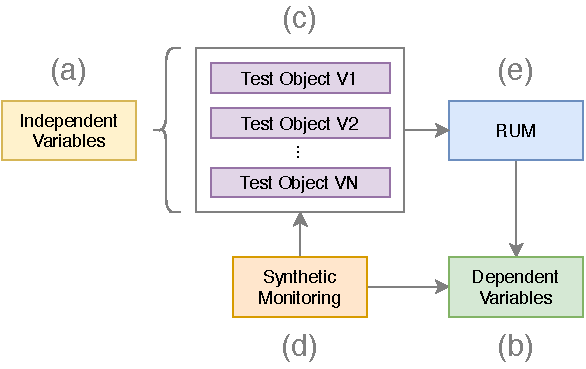
\includegraphics[width=0.8\textwidth]{design.pdf}
\caption{Components from the Controlled Experiment}
\label{figure:design_setup}
\end{center}
\end{figure}

The different parts of the experiment setup will be discussed in more detail below.


% Kohavi 2016: Sample size, collect right metrics, track right users, randomization unit


% --------------------------------------------------

\subsection{(a) Independent Variables}

% [What are they representing]

The IVs reflect two things:
How the tracking script is included into the website, and if another tracking script is present or not.
All IVs and the values they can take are listed in table X:

As described in section X, page tagging is the method of choice when including a tracking script into a website.
Page tagging is in essence the addition of a <script>-Tag to the main HTML document.
Different options exist when adding a script to the main document.
IV 1 describes the the position of the tracking script within the main document.
IV 2 describes the attribute of the included script tag.

If another tracking script, which may interfere with the "main" tracking script, is presented in the main document or not, is reflected in IV 3.

\begin{table}[h]
	\small
	\centering
	\begin{tabular}{ | l | l | l | }
	\hline
	IV \cellcolor{lightgrey} & Describes \cellcolor{lightgrey} & Possible Values \cellcolor{lightgrey} \\
	\hline
	1 & Position of the Tracking Script & top-head, bottom-head, bottom-body \\
	2 & Attribute of the Tracking Script & none, async, defer \\
	3 & Other Tracking Script included & no, yes \\
	\hline
	\end{tabular}
	\medskip
	\caption{Independent Variables}
	\label{table:independent_variables}
\end{table}


The three IVs are discussed in more detail in the following.
Other IVs considered, but not incorporated within the experiment, are discussed in section X.

% -------------------------

\subsubsection{IV 1: Position of the Tracking Script}

% [GA Tracking Code]

This IV may help understand if the position of the tracking script affects the performance.
Google Analytics (GA) is used as the tracking script.
In general, scripts can be included within the head or body section of the HTML document. % https://www.w3schools.com/js/js_whereto.asp
The GA documentation suggests that the GA script "should be added near the top of the <head> tag and before any other script or CSS tags".
% cite https://developers.google.com/analytics/devguides/collection/analyticsjs
Some details about the GA script are given in section X.

% [Other examples]

Other RUM vendors propose a similar position:
Hotjar suggests that "Paste the Tracking Code into the <head> section of your website."
And Akamai says for there tracking tool boomerang:
"Paste the following code snippet into every page of your site at the top of the HEAD, but after sensitive META tags."
% https://developer.akamai.com/tools/boomerang#dealing-with-script-error

The three possible positions of the tracking script, top-head, bottom-head, and bottom-body, are visualized in appendix X.


% https://speedcurve.com/setup/lux/
% SpeedCurve tracking script position: To add real user monitoring (RUM) to your site, paste this snippet at the top of the <HEAD> tag on your pages.

% Grigorik Conference Talk https://www.youtube.com/watch?v=PkOBnYxqj3k&ab_channel=IlyaGrigorik
% And slides https://www.igvita.com/slides/2013/fluent-perfcourse.pdf


% -------------------------

\subsubsection{IV 2: Attribute of the Tracking Script}

The IV 2 is about the attribute of tracking script tag.
As explained in section X, possible attributes, next to have no attribute, are async and defer, and attributes are not applied on inline scripts.

As the GA script is included inline, different attributes should not affect the behaviour of the website nor its performance.
This IV should verify if this statement holds true and it is expected that changing this variable has no impact on performance.

The three attributes none, async, and defer are visualized in appendix X.


% -------------------------

\subsubsection{IV 3: Other Tracking Script is included}

Many websites use more than one tracking script to collect user data or even resort to custom tracking solutions.
Adding and loading another script within the website will increase the page weight, which leads to more requests and bytes, and depending for example on the network speed, loading an additional resource may impact performance badly.

The other script should not be any kind of script, but also a RUM solution, which has the objective to collect and report user data.
This IV is binary and models if another tracking script is included or not.
Changing this variable may capture if multiple tracking scripts interfere with each other.

Hotjar will be used as the additional tracking script.
The two variants, one with an additional script and one without, are visualized in appendix X.

% footnoe hotjar

% -------------------------

\subsubsection{Other IVs not considered but worth mentioning}

Many other IVs could be chosen and they could reflect variables of the tracking script itself, the website, or the infrastructure around it.

% [Script]

As for the additional IVs for the tracking script, other variables could reflect the quality or complexity of the tracking script, e.g., what kind of user data is collected and in what quantity.
Other variables may reflect the file size of the script, or compare different versions and implementations of the same RUM script.

% [Website]

Possible variables for the website may reflect implementation details, how the code is structured, which libraries are used, how many resources such as images and videos are being loaded, how they are arranged, how the CSS is handled, etc.

% [Infrastructure]

And in terms of infrastructure, IVs may model which servers are being used, which webservers run on them, the condition of the network, the device of the end users, or his operating system, browser version, and so on.
Especially on a website and infrastructure level, nearly countless IVs are imaginable.


% -------------------------

\subsubsection{Possible Variations of the Independent Variables}

% [Variants]

When putting the three defined IVs "Position", "Attribute", and "Other Script" together, different possible combinations emerge as displayed in table X.
The variants A1 and OS2 are redundant and will be dismissed as their IV configuration is already represented in variant P1.

\begin{table}[h]
	\small
	\centering
	\begin{tabular}{  | c || c | c | c | } 
	\hline
	Variant & Position & Attribute & Other Scripts \\
	\hline \hline
	Variant P1 & top-head & \cellcolor{lightgrey} none & \cellcolor{lightgrey} no \\
	   Variant P2 & bottom-head & \cellcolor{lightgrey} none & \cellcolor{lightgrey} no \\
	   Variant P3 & bottom-body & \cellcolor{lightgrey} none & \cellcolor{lightgrey} no \\
	  \hline
	   \sout{Variant A1} & \cellcolor{lightgrey} \sout{top-head} & \sout{none} & \cellcolor{lightgrey} \sout{no} \\
	   Variant A2 & \cellcolor{lightgrey} top-head & async & \cellcolor{lightgrey} no \\
	   Variant A3 & \cellcolor{lightgrey} top-head & defer & \cellcolor{lightgrey} no \\
	  \hline
	  \sout{Variant OS1} & \cellcolor{lightgrey} \sout{top-head} & \cellcolor{lightgrey} \sout{none} & \sout{no} \\
	  Variant OS2 & \cellcolor{lightgrey} top-head & \cellcolor{lightgrey} none & yes \\
	  \hline
	\end{tabular}
	\medskip
	\caption{Possible Test Object Variants when combining the IVs.}
	\label{table:test_object_variants}
\end{table}


% [What are the Variants]

The variants themselves are different index.html files from the test website.
The difference between the variants are only the options and position of the tracking script, as described above.
The rest of the test website is remaining the same over all variants.
How the test website is constructed, is discussed below.

% [Evaluation/Comparison]

For evaluation, I will compare the different possible values of one IV with each other, while the values of the other IVs remain unchanged.
For example, the different positions (IV 1) are compared with each other, while the attribute (IV 2) and whether or not another script is included (IV 3) remain the same for all positions.
This is needed in order to measure the impact when changing one IV.
Variants which are not from the same subgroup are not compared with each other, e.g. variant A2 will not be compared to variant OS2.


% --------------------------------------------------

\subsection{(b) Dependent Variables}

The dependent variables measure the outcome of the change in IVs with respect to web performance.
They are web performance metrics.
The synthetic monitoring and RUM solutions implemented in the experiment measure and deliver the dependent variables.

The dependent variables are visualized in order to facilitate the interpretation of the data.
Considered dependent variables (web performance metrics) are common web performance metrics as described in section X, such as page weight, navigation timing metrics such as TTFB and PLT, and user-centric metrics such as Speed Index or LCP.


% -------------------------------------------------------------------------
% -------------------------------------------------------------------------

\subsection{(c) The Test Object: An E-Commerce Website}

% [Difficulty]

In the real world, each website is unique and follows its own design and architecture principles.
The difficulty for conducting research on websites such as within this thesis, is to find a common ground or general website that approximates real world examples as good as possible.

%TODO add best would be real life scenario ?

% Mimic the website is one thing, but also all other aspects should be fairly similar: infrastructure (hosting), hardware used, network speed, traffic, etc.
% This experiment/test is only an approximation and can serve as a starting point for further investigations

% Ideal: Use a real website. Is not possible


% [Goal]

One goal of this thesis is to create a test website which mimics a real life e-commerce website as good as possible.
Multiple ideas to achieve this goal are presented and discussed in the following.


% --------------------------------------------------------

\subsubsection{Minimal Website}

% [Idea]

The idea of the minimal website is to have a clean, laboratory-like environment which is in full control of the tester.
The minimal website is constructed without any content but only a link to an external script, which represents the tracking script.
The script itself has only place holder content which adds bytes to the file size, but does not execute any logic.
    
% [Setup]

The website is hosted, like all following test websites, on GitHub Pages, which is a quick, easy and fast way to deploy a website onto a real server.
The source code for the minimal website is available on GitHub, and the page is deployed to https://aramovski.github.io/.
% footnote : https://github.com/aramovski/aramovski.github.io
% Footnote https://pages.github.com/ [30.08.2021]

% [Evaluation]

The benefit of this approach is that the tester has a lot of control about the website, as there are not many complex coherences or variables within the website itself.
The three discussed IVs can easily be changed.
In addition, the script file size can be changed quickly.
As a downside, the minimal website is too far away from any real world website, e.g. no images or other resources are requested.
Also, it does not cover any e-commerce scenario.
Hence, this idea has been withdrawn.


% --------------------------------------------------------

\subsubsection{Median Website}

% [Idea]

The idea of the median website is to construct a website which represents an "average" website as good as possible in order to cover as many real life examples as possible.
The median website is created with a median page weight.
This means, it has an average amount of requests and bytes for each resource type such as images, fonts, or videos.
The data for the median values is taken from HTTPArchive. %footnote
The source code is available on GitHub and the page is deployed to https://aram-yesildeniz.github.io/median/.
%footnote source. https://github.com/aram-yesildeniz/median/tree/gh-pages

% [Evaluation]

The evaluation of the median website idea leads to the conclusion that this approach could only serve as a proof of concept or initial iteration for environment or other contextual components testing.
Additionally, it could serve as a basis for questions regarding page weight only.
The architecture of the median website is artifial, e.g. all resources are loaded in sequence.
There is no dynamic content, no navigation items or sub-pages, and no resemblance to an e-commerce website.
In short, the median website is too far away from reality.


% 2011 Grigorik Anatomy of modern web application
% - Chart with changes on time: apps are growing

% 2014 Hogan basics-of-page-speed/ What Is the HTTP Archive?


% --------------------------------------------------------

\subsubsection{WordPress Website}

% [Idea]

The idea of the WordPress website is to leverage one of the most widely used website building frameworks in order to cover many real world examples, which also rely on this content management system.
WordPress is roughly used by 40% of all websites.
% footnote https://w3techs.com/technologies/details/cm-wordpress

% [Plugins]

WordPress follows a plugin system which allows the operators of the website to easily integrate new features and tools into the website.
WooCommerce, an e-commerce plugin, is the most widely used plugin and used by nearly a fifth of all websites running on WordPress.
% footnote https://w3techs.com/technologies/details/cm-wordpress

% [Setup]

The WordPress website is constructed by downloading the latest version of WordPress and running it on the local webserver MAMP.
The idea of running the website on localhost is that it gives more control to the tester.
% footnote https://wordpress.org/download/
% footnote https://www.mamp.info/de/mac/
Additionally, WooCommerce and Google Analytics are integrated as plugins into the website.
Finally, WebPageTest is configured to measure and generate traffic for the website running on localhost.
%footnote https://www.monsterinsights.com/

% [Evaluation]

The idea of running WordPress on localhost was withdrawn:
Although the generated pages and templates from WordPress approximated real life websites, they could not compensate missing content and resources such as images or stylesheets.
As with the approaches described above, the WordPress website is too far away from a real life scenario.

%The rather unconventional setup to run WordPress on localhost and not on a common webhosting service.


% --------------------------------------------------------

\subsubsection{Mirroring a complete e-commerce website}

% [Idea]

The three approaches described above all have the same problem: they do not get sufficiently close to mimic real websites.
To counter attack this issue, the idea of mirroring a complete e-commerce website evolved, with the aim to approximate reality as close as possible.
Candidates for cloning are e-commerce websites with the biggest revenue in Germany.
% footnote https://de.statista.com/statistik/daten/studie/170530/umfrage/umsatz-der-groessten-online-shops-in-deutschland/
The first candidate is https://www.otto.de/, which is discarded as discussed below.
The second candidate https://www.zalando.de/ is used as the test object for the experiment.
Both, Otto and Zalando, are within the top three of e-commerce websites with highest revenue.

% [Setup]

Multiple tools exist to clone, mirror or download a complete website.
Tools used here are HTTrack and the Google Chrome extensions "Save All Resources".
As with the other approaches, the downloaded website will then be hosted on GitHub Pages.
% footnote https://www.httrack.com/
% footnote https://chrome.google.com/webstore/detail/save-all-resources/abpdnfjocnmdomablahdcfnoggeeiedb?hl=en


% --------------

\paragraph{Otto}

% [Manual Adjustments]

The naive approach is to download https://www.otto.de/ via HTTrack and move the content to GitHub Pages, which serves the website.
Some issues evolved with this approach, which were mostly cookie related issues and probably dynamic created resources, that could not be found and served.
This caused the web server to return more than a few 404s.

Additionally, problems with caching in combination with WebPageTests repeat view feature occurred:
The free webhosting service offered by GitHub does not allow to configure the webserver.
Especially caching in terms of HTTP cache-control headers can not be adjusted.
Therefore, the webserver decides which resources should be cached by the browser.
The configuration is such that many resources served will be cached by the browser.
This behaviour differs from the behaviour found on https://www.otto.de/, where caching is disabled for many resources, and resources will be downloaded again from the server also for repeat views.
The problem is not only that caching behaviour differs between the test object and the original website, but also that WebPageTests repeat view runs are failing when encountering too many missing resources.
Hence, data for repeat views is corrupt and can not be collected.

% Add Workaround ?
% Therefore i mock the missing ressources so that WPT can run bulk tests successfully.
% It is not possible to change the github request headers. We can modify the http request headers via html, but this is not a clean solution.
% Not possible to set cache control in html meta tag https://html.spec.whatwg.org/multipage/semantics.html#attr-meta-http-equiv


% [Evaluation]

Due to the caching problems and the failing repeat view runs in WebPageTest, this approach was declined.
Ideally, the test website is hosted on a similar infrastructure like the original website, with similar webserver configurations.
For economic and effort reasons this is not feasible, therefore another original website to clone with less caching issued has to be taken into account.

[more here ?]

% - user-set-consent-id-cookie: Cookie with name consentId is not set, user-set-consent-id-cookie returns therefore 404
% - subscribeToNewsletterSnippetContent: Change path did not work...
% - amount.json: Not found, also wl\_miniWishlistAmount in local storage does not created
% - a\_info: Mock a\_info response json does not work...

% - footer not visible
% - userTiming


% - mock image sprite\_all\_1ba408b2.png
% - create empty file called user-set-consent-id-cookie
% - change path for subscribeToNewsletterSnippetContent: This will remove the cookie banner... but then WPT works


% -------------------

%TODO add Compare original otto website with mock ?
% \subparagraph{Comparison to original webpage}
% Maybe use here just WPTs comparison tool
% Show some diagrams here
% The other diagrams with Zalando should go into evaluation chapter


% --------------------------------------------------------

\paragraph{Zalando}

% [Why]

For https://www.zalando.de/, the cache control configuration of the webserver differs and the issues of caching and repeat views are not occurring.
This makes the website easier to clone and the favourite candidate to serve as the test object.

% [Setup]

The website is downloaded via the "Save All Resources" Chrome extension and the content is uploaded to GitHub, from where it will be served through GitHub Pages.
The source code of the test website is published at GitHub and the website is accessible at https://aram-yesildeniz.github.io/.
% footnote https://github.com/aram-yesildeniz/aram-yesildeniz.github.io
How the test website differs from the original website is shown in the next chapter.
Figure X provides screenshots from the original and the test website.

\begin{figure}
	\centering
	\begin{subfigure}{.5\textwidth}
		\centering
		
\includegraphics[width=1\linewidth]{original_screenshot.png}
		\caption{https://www.zalando.de/}
		\label{fig:sub1}
	\end{subfigure}%
	\begin{subfigure}{.5\textwidth}
		\centering
		
\includegraphics[width=1\linewidth]{test_screenshot.png}
		\caption{https://aram-yesildeniz.github.io/}
		\label{fig:sub2}
	\end{subfigure}
	\caption{Original vs Test Object}
	\label{figure:zalando_original_test}
\end{figure}


Table X summarizes the discussed approaches.


\begin{table}[h]
	\small
	\centering
	\begin{tabular}{ | l | l | c | c | }
%	\begin{tabular}{ | p{0.3\linewidth} | p{0.6\linewidth} | }
	\hline
	\cellcolor{lightgrey} Idea & \cellcolor{lightgrey} Template & \cellcolor{lightgrey} Complexity & \cellcolor{lightgrey} Close to Reality \\
	\hline
	Minimal & Basic HTML Template & - & - \\
	Median & HTTPArchive & + & + \\
	WordPress & WordPress Default & ++ & + \\
	Clone & E-Commerce Website & ++ & +++ \\
	\hline
	\end{tabular}
	\medskip
	\caption{Approaches Summary}
	\label{table:performance_metrics_conclusion}
\end{table}


% --------------------------------------------------


\subsection{(d) Synthetic Monitoring: Create Traffic and Collect Data}

The Synthetic Monitoring component within the experiment design has two functions:
One, it measures the performance of the website, and two, it generates traffic on the website, which is needed in order for RUM to measure data.

% This setup is a special case because lab bots (e.g. WPT) simulate at the same time real users for RUM data


% \subsubsection{WebPageTest}

% [Setup]

WebPageTest (WPT) is used as the synthetic monitoring component.
Multiple options of using WPT exist:
The quickest way is to use the public version which is available at https://www.webpagetest.org/.
Due to long waiting times, and possible fluctuations for example in peak hours, this option is not suitable.
Another option is to programmatically use the public version via the public API.
This option is not feasible as the API is throttled by limits and quotas.

WPT is open source and can be downloaded and run in private instances.
One option of running a private instance is by using a preconfigured Amazon Machine Image which runs within the Amazon Cloud.
This option is disregarded due to financial aspects.
The most affordable and also most controllable approach is to run WPT on localhost.
For the experiment, a private instance of WPT running on localhost within a Docker environment is used.
% footnote: Guide: https://medium.com/@francis.john/local-webpagetest-using-docker-90441d7c2513

% [Configuration]

As described in section X, WPT is highly configurable.
The configuration for this experiment is described in table X.

[more here?]

\begin{table}[h]
	\small
	\centering
	\begin{tabular}{  | l | l | } 
	\hline
	\cellcolor{lightgrey} Configuration Setting & \cellcolor{lightgrey} Option \\
	\hline
%	Test Location & Test Location \\ 
	Browser & Chrome \\
	Connection & LAN (connection speed is determined by hotspot) \\
	Desktop Browser Dimensions & default (1366x768) \\
	Number of Tests to Run & 1 \\
	Repeat View & First View and Repeat View \\
	Capture Video & True \\
	Keep Test Private & False \\
	Label & none \\
	\hline	  
	Advanced Tab & Nothing selected \\
	Chromium Tab & Capture Dev Tools Timeline selected  \\
	Auth, Script, Block, SPOF, Custom Tabs & Nothing  \\
	Bulk Testing Tab & URL of the test website $x$ times according to test plan \\
	\hline
	\end{tabular}
	\medskip
	\caption{WPT Configuration}
	\label{table:wpt_configuration}
\end{table}


% [FV vs RV] ??

% First View: "First View refers to the cold cache setup in which nothing is served locally"
%Repeat View: "Repeat View refers to the warm cache containing everything instantiated by the first view" (2016 Using WPT p. 62)


% ----------------------

\paragraph{Traffic Shaping}

% [Why]

The network condition has a not negligible role in web performance, as described in section X.
For reliable and comparable data, it is important to keep the network connectivity stable and similar over all test runs (see also X).
In general, exactly which bandwidth and latency is chosen for the test is secondary, as long as the configuration remains the same for all test runs.
% cite https://calendar.perfplanet.com/2016/testing-with-realistic-networking-conditions/

% [Solutions]

WPT ships with a traffic shaping functionality.
Unfortunately, this functionality is not available when running a private WPT instance on Docker on macOS (the localhosts OS).
Hence, the network connection of the whole machine has to be throttled.
This can be achieved through a software or hardware solution:

The software solution is to use a tool like Network Link Conditioner to slow down the whole machine.
This tool is also suggested by the developer of WPT. % cite blogpost
% footnote https://nshipster.com/network-link-conditioner/
Spot tests indicate that this solution is not that reliable and the internet speed still varies.
Therefore in the experiment, a hardware solution is chosen.
The network condition relies on a mobile hotspot device which is throttled to 50 mbit/s.

% Overview table with different settings:
% https://developer.mozilla.org/en-US/docs/Web/Performance/Understanding_latency

% WPT also slows down their whole machines https://forums.webpagetest.org/t/measure-internet-speed/11593

% i will use the durchschnitt in germany which seems to be 40 mbit per second. or actually i use LTE profile from network conditioner which is 50 mbit per second 

% ----------------------

\paragraph{Usage of the Bulk Test Feature}

As will be discussed in section X, the synthetic monitoring component should not only measure the test website once, but multiple times.
The private instance of WPT offers a feature called Bulk Test, which enables the tester to pass a list of URLs to the test agent which processes the list in one go.
This feature is used to trigger multiple test runs.
When completed, the measured data is collected over all tests and summarized in one csv file, which is downloaded and used for further analysis.

% keep in mind that FV and RV for one test are directly next to each other
% so to get data for all FVs, i would need data from rows 1 3 5 etc


% --------------------------------------------------


\subsection{(e) Real-User Monitoring: Google Analytics}

RUM is integrated into the test website to measure data and on the same time represents the tracking script on which the IV are applied to.
Google Analytics is used and integrated into the website with the code snippet in listing X.

% [Code explanation]

[Explain Code]

% Set sample rate to 100% for speed metrics

% https://developers.google.com/analytics/devguides/collection/analyticsjs/


% Actually, it creates another async script tag which loads the actual analytics JS.
% So basically it should not really play a role where we place it.
% Basically the sync part is only..
% It creates another script tag which is async and which loads the tracking code.

% Meaning for IV Attribute:
% This script is an inline script, as it does not have any src attribute.
% In theory,  async and defer attributes on inline scripts are ignored, as explained in section X.
% "Inline JavaScript script tags ignore the defer or async attribute"
% As the "wrapper" snippet is a inline script (no src attribute), the attributes on this script tag should not have any effect.

% Evaluation will show.


\begin{center}
\begin{lstlisting}[caption={The Google Analyitcs Tracking Script}, label={listing:ga_script}, numbers=none]
<!-- Google Analytics -->
<script>
  (function (i, s, o, g, r, a, m) {
    i['GoogleAnalyticsObject'] = r;
    i[r] = i[r] || function () {
      (i[r].q = i[r].q || []).push(arguments)
    }, i[r].l = 1 * new Date();
    a = s.createElement(o), m = s.getElementsByTagName(o)[0];
    a.async = 1;
    a.src = g;
    m.parentNode.insertBefore(a, m)
  })
  (window, document, 'script',
   'https://www.google-analytics.com/analytics.js', 'ga');

  ga('create', {
    trackingId: 'UA-XXXXXXXXX-X',
    cookieDomain: 'auto',
    siteSpeedSampleRate: 100
  });
  
  ga('send', 'pageview');
</script>
<!-- End Google Analytics -->
\end{lstlisting}
\end{center}


% [Data Collection]

The data is available through the Google Analyitcs dashboard.
To get quicker access to the data and only fetch the data needed, which is about site speed, I use a helper tool which uses the API to retrieve the data.
The source code of the helper tool is on GitHub and deployed to https://aram-yesildeniz.github.io/google-analytics/.
% footnote https://github.com/aram-yesildeniz/google-analytics


% ------------------------------------------------------------------------------------------
% ------------------------------------------------------------------------------------------

\section{Conducting the Experiment}

All variants are tested according to the plan in table X.
For each test run, I follow a rigorous testing procedure to eliminate possible careless mistakes (table X).

\begin{table}[h]
	\small
	\centering
	\begin{tabular}{ | l | l | l | l | } 
	 \hline
	  Variant \cellcolor{lightgrey} &  Date \cellcolor{lightgrey} & Traffic Shaping \cellcolor{lightgrey} & Runs \cellcolor{lightgrey} \\
	  \hline
	  Original Website & 2021-05-28 & 50 Mbit/s & 500 \\
	  Test Website without GA included & 2021-05-29 & " & " \\
	  \hline
	  Variant P1 & 2021-05-30 & " & " \\
	  Variant P2 & 2021-05-31 & " & " \\
	  Variant P3 & 2021-06-02 & " & " \\
	  \hline
	  Variant A2 & 2021-06-04 & " & " \\
	  Variant A3 & 2021-06-09 & " & " \\
	  \hline
	  Variant OS2 & 2021-06-03 & " & " \\
	  \hline
	  \end{tabular}
	\medskip
	\caption{Test Plan}
	\label{table:test_plan}
\end{table}


\begin{table}[h]
	\small
	\centering
	\begin{tabular}{ | p{0.1\linewidth} | p{0.8\linewidth} | } 
	\hline
	Step \cellcolor{lightgrey} & Task \cellcolor{lightgrey} \\
	1 & Deploy the required variant of test website by pushing the specific index.html file to GitHub \\
% \item Start Network Link Conditioner with specified config on local machine
	2 & Verify that the internet speed of test machine is around 50 mbit/s (by using speedtest-cli) \\
	3 & Start the private Docker instance of WebPageTest on localhost \\
	4 & Set the WebPageTest configuration according to the predefined configuration and add the list of URLs to bulk test interface \\
	5 & Start the test run \\
	6 & When testing is done, download the summary csv file which contains all relevant data \\
	7 & On the GA helper site, download the measured data for the current day \\
	\hline
	\end{tabular}
	\medskip
	\caption{Test Run Checklist}
	\label{table:test_run_checklist}
\end{table}
% footnote https://www.speedtest.net/apps/cli

% [Data Collection]

As described, the data used for further analysis is downloaded from the WebPageTest test summary page and from the GA helper site.
The evaluation and analysis of the data is subject of the next chapter.